\chapter{Construction}

\section{Mobilization} 

Construction mobilization continues, with a total of 750 personnel on Site. We expect another 200 tradesmen with the next 15 days, as more materials and areas open up.

\section{Basement Works}

Large areas of B4, B3 have now been handed over to Conspel. We have started works for drainage, fire-fighting and electrical second fix installations. Mock-ups for riser installations are in progress and once approved we expect to add personnel to accelerate the works.

Progress is still in small percentages, as it is reported by value. 

\section{Subcontractors}

The Commissioning Management subcontractor has now been approved (AJB). This has been resubmitted also for TAB.

\section{Material Deliveries}

Material deliveries to site continue. Current problematic deliveries are deliveries for cable trays and accessories. Remedial measures have been
taken to submit a local supplier with better delivery schedules. These are expected to start within 20 days, giving time for approvals, ordering
and issuing of any financial documents.

Fire Fighting materials are now in place, with piping, supports, couplings all start arriving. We expect good progress of the Fire Fighting works
thereafter.

\begin{figure}[htbp]
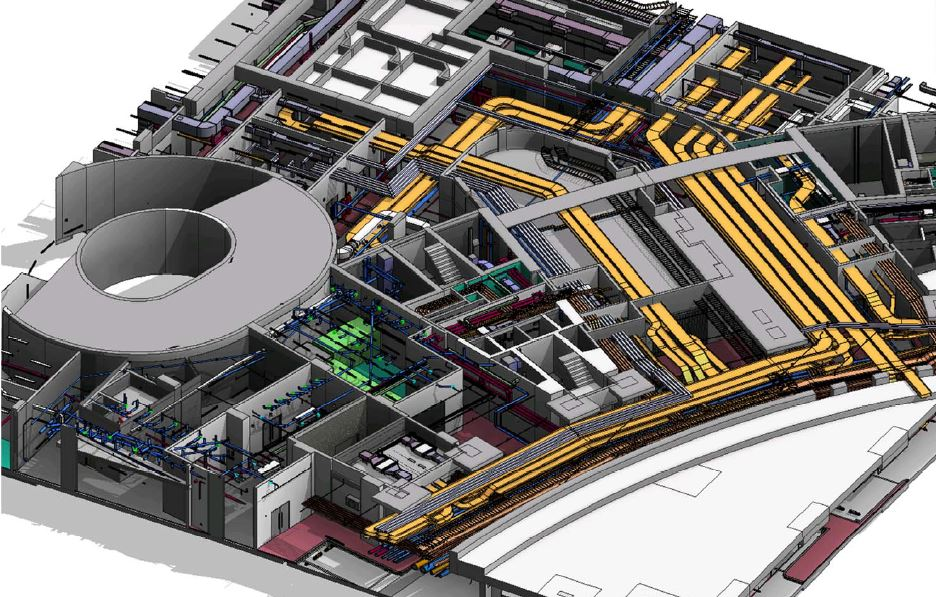
\includegraphics[width=\textwidth]{B1-BIM}
\end{figure}

\section{Encodings}

In an infamous post on stackoverflow user ... posted the below snippet\ldots

\begin{quotation}
You can't parse [X]HTML with regex. Because HTML can't be parsed by regex. Regex is not a tool that can be used to correctly parse HTML. As I have answered in HTML-and-regex questions here so many times before, the use of regex will not allow you to consume HTML. Regular expressions are a tool that is insufficiently sophisticated to understand the constructs employed by HTML. HTML is not a regular language and hence cannot be parsed by regular expressions. Regex queries are not equipped to break down HTML into its meaningful parts. so many times but it is not getting to me. Even enhanced irregular regular expressions as used by Perl are not up to the task of parsing HTML. You will never make me crack. HTML is a language of sufficient complexity that it cannot be parsed by regular expressions. Even Jon Skeet cannot parse HTML using regular expressions. Every time you attempt to parse HTML with regular expressions, the unholy child weeps the blood of virgins, and Russian hackers pwn your webapp. Parsing HTML with regex summons tainted souls into the realm of the living. HTML and regex go together like love, marriage, and ritual infanticide. The <center> cannot hold it is too late. The force of regex and HTML together in the same conceptual space will destroy your mind like so much watery putty. If you parse HTML with regex you are giving in to Them and their blasphemous ways which doom us all to inhuman toil for the One whose Name cannot be expressed in the Basic Multilingual Plane, he comes. HTML-plus-regexp will liquify the n​erves of the sentient whilst you observe, your psyche withering in the onslaught of horror. Rege̿̔̉x-based HTML parsers are the cancer that is killing StackOverflow it is too late it is too late we cannot be saved the trangession of a chi͡ld ensures regex will consume all living tissue (except for HTML which it cannot, as previously prophesied) dear lord help us how can anyone survive this scourge using regex to parse HTML has doomed humanity to an eternity of dread torture and security holes using regex as a tool to process HTML establishes a breach between this world and the dread realm of c͒ͪo͛ͫrrupt entities (like SGML entities, but more corrupt) a mere glimpse of the world of reg​ex parsers for HTML will ins​tantly transport a programmer's consciousness into a world of ceaseless screaming, he comes, the pestilent slithy regex-infection wil​l devour your HT​ML parser, application and existence for all time like Visual Basic only worse he comes he comes do not fi​ght he com̡e̶s, ̕h̵i​s un̨ho͞ly radiańcé destro҉ying all enli̍̈́̂̈́ghtenment, HTML tags lea͠ki̧n͘g fr̶ǫm ̡yo​͟ur eye͢s̸ ̛l̕ik͏e liq​uid pain, the song of re̸gular exp​ression parsing will exti​nguish the voices of mor​tal man from the sp​here I can see it can you see ̲͚̖͔̙î̩́t̲͎̩̱͔́̋̀ it is beautiful t​he final snuffing of the lie​s of Man ALL IS LOŚ͖̩͇̗̪̏̈́T ALL I​S LOST the pon̷y he comes he c̶̮omes he comes the ich​or permeates all MY FACE MY FACE ᵒh god no NO NOO̼O​O NΘ stop the an​*̶͑̾̾​̅ͫ͏̙̤g͇̫͛͆̾ͫ̑͆l͖͉̗̩̳̟̍ͫͥͨe̠̅s ͎a̧͈͖r̽̾̈́͒͑e n​ot rè̑ͧ̌aͨl̘̝̙̃ͤ͂̾̆ ZA̡͊͠͝LGΌ ISͮ̂҉̯͈͕̹̘̱ TO͇̹̺ͅƝ̴ȳ̳ TH̘Ë͖́̉ ͠P̯͍̭O̚​N̐Y̡ H̸̡̪̯ͨ͊̽̅̾̎Ȩ̬̩̾͛ͪ̈́̀́͘ ̶̧̨̱̹̭̯ͧ̾ͬC̷̙̲̝͖ͭ̏ͥͮ͟Oͮ͏̮̪̝͍M̲̖͊̒ͪͩͬ̚̚͜Ȇ̴̟̟͙̞ͩ͌͝S̨̥̫͎̭ͯ̿̔̀ͅ
\end{quotation}

The argument was that one could not use Regular Expressions to parse HTML. In reality parsing wild HTML is very difficult as browsers aim to render text even if there is malformed HTML, with many healing algorithms employed. When Knuth designed TeX, the parsing was all handcrafted. He did not automate any parts of it.

